\documentclass[../ZF_SWEN1.tex]{subfiles}

\begin{document}
\begin{figure}[H]
\centering
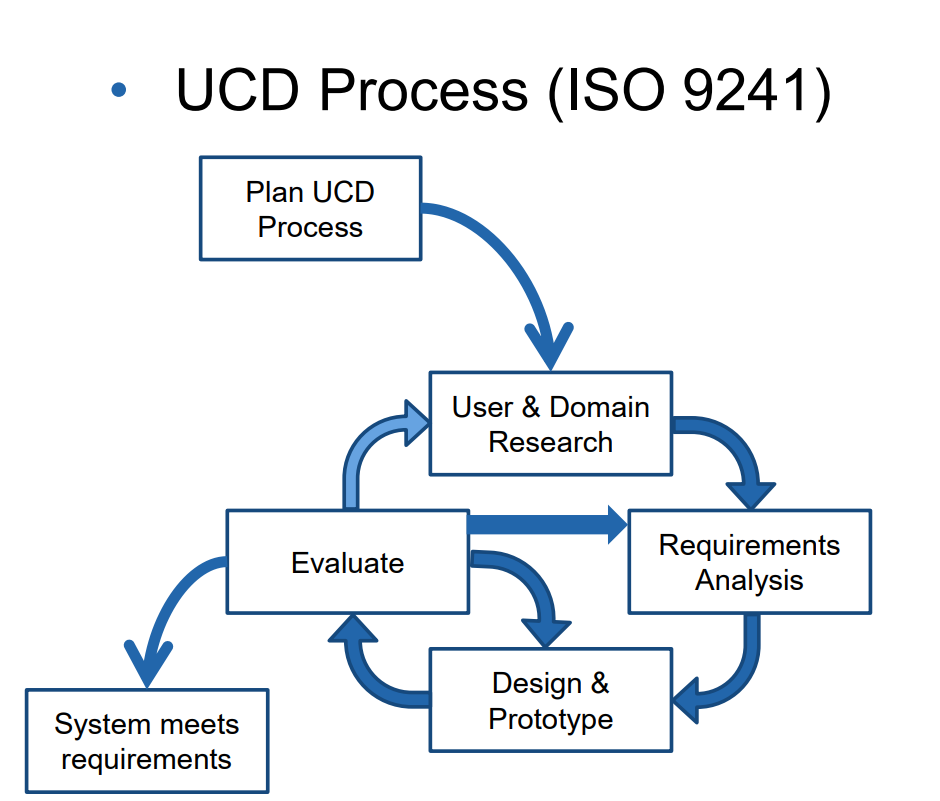
\includegraphics[width=0.3\textwidth]{Resources/Images/UCD_Process.png}
\caption{\label{fig:UCDProcess} UCDProcess}
\end{figure}


\subsection{User \& Domain Research}
\begin{itemize}
	\item \textcolor{red} {\textbf{Ziele bez. Benutzer:}}
	\begin{itemize}
		\item Wer ist Benutzer
		\item Was ist die Arbeit (Aufgaben, Ziele)
		\item Wie sieht Arbeitsumgebung aus
		\item Was wird gebraucht um Ziele zu erreichen
	\end{itemize}
	\item Welche Sprache, Begriffe
	\item Normen (organisatorisch, kulturell, sozial)
	\item Pain Points (Brüche, Workarounds)
	\item Für mobile Apps:
	\begin{itemize}
		\item Nutzungskontext
		\begin{itemize}
			\item Wo wird App benutzt (Umgebung)
			\item Wann wird App benutzt (Tageszeit, involvierte Personen, Randbedingungen)
			\item Warum wird App benutzt (Nutzen, Motivation, Trigger)
		\end{itemize}
	\end{itemize}
	\item \textcolor{red} {\textbf{Ziele bez. Domäne:}}
	\begin{itemize}
		\item Buisiness der Firma verstehen
		\item Domäne verstehen (Sprache, Wichtigste Konzepte, Prozesse)
	\end{itemize}
	
\end{itemize}




\subsubsection{GUI Design Process}
\paragraph{Methoden User \& Domain Research}
\begin{itemize}
	\item Contextual Inquiry
	\item Interviews
	\item Beobachtung
	\item Fokusgruppen
	\item Umfragen
	\item Nutzungsauswertung
	\item Desktop Research (Dokumentenstudium, Mitbewerber)
\end{itemize}


\subsubsection{Wichtige Artekfakte}
\begin{itemize}
	\item \textcolor{pink}{\textbf{Personas}}
	\item \textcolor{pink}{\textbf{Usage-Szenarien}}
	\begin{itemize}
		\item Kurze Geschichte
		\begin{itemize}
			\item \textcolor{green} {Usage Szenarien}
			\begin{itemize}
				\item aktuelle Situation
				\item in User and domain research verwendet
			\end{itemize}
			\item \textcolor{green} {Kontextszenarien}
			\begin{itemize}
				\item Zukünftige gewünschte Situation
				\item in Anforderungsanalyse verwendet
			\end{itemize}
		\end{itemize}
		
	\end{itemize}
	\item \textcolor{pink}{\textbf{Mentales Modell}}
	\item \textcolor{pink}{\textbf{Domänenmodell}}
	\item \textcolor{pink}{\textbf{Stakeholder Map}}
	\begin{figure}[H]
	\centering
	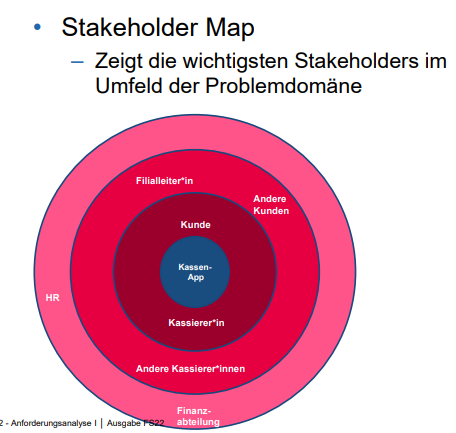
\includegraphics[width=0.3\textwidth]{Resources/Images/Stakeholdermap.png}
	\caption{\label{fig:Stakeholdermap} Stakeholdermap}
	\end{figure}
	\item \textcolor{pink}{\textbf{Service Blueprint/Geschäftsprozessmodell}}
	\begin{figure}[H]
	\centering
	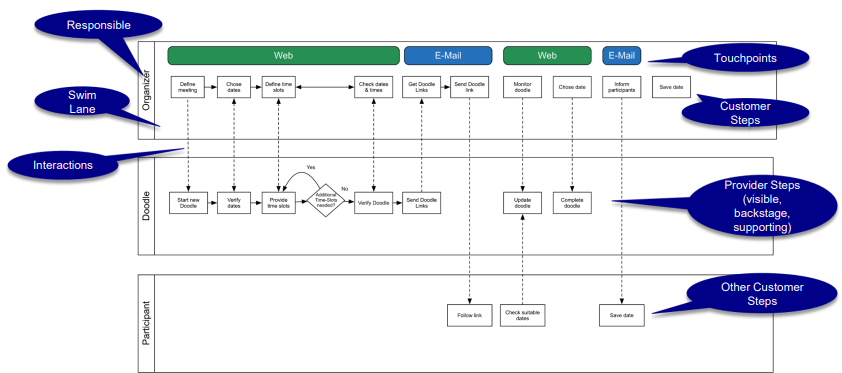
\includegraphics[width=0.3\textwidth] {Resources/Images/Blueprint.png}
	\caption{\label{fig:Blueprint}Blueprint}
	\end{figure}
	
\end{itemize}

\subsection{Anforderungsanalyse}

\textbf{Ziel:}\\
\begin{itemize}
	\item Ausgehend von den Resultaten des UCD -> User-Anforderungen ableiten:
	\begin{itemize}
		\item Funktionale Abläufe, Interaktionen 
		\begin{itemize}
			\item \textcolor {gray} {\textbf{Kontextszenarien}}
			\item \textcolor {gray} {\textbf{Storyboards}}
			\item \textcolor {gray} {\textbf{UI-Skizzen}}
			\item \textcolor {gray} {\textbf{Use cases}}
		\end{itemize}
		\item Konzepte, Beziehungen, Quantitäten
		\begin{itemize}
			\item \textcolor {gray} {\textbf{Kontextszenarien}}
		\end{itemize}
		\begin{itemize}
			\item \textcolor {gray} {\textbf{FURPS-Modell (Functionality, Usability, Reliability, Performance, Supportablility}}
		
		\end{itemize}				
		
	\end{itemize}
\end{itemize}


\subsubsection{Use Cases}

\begin{itemize}
	\item Akteur
	\begin{itemize}
		\item Primärakteur
		\item Unterstützender Akteur
		\item Offstage-Akteur
	\end{itemize}
	\item Keine Kann-Formulierungen
	\item 3 Ausprägungen:
	\begin{itemize}
		\item Kurz
		\begin{itemize}
			\item Titel + 1 Absatz (Standardablauf)
		\end{itemize}
		\item Informell
		\begin{itemize}
			\item Titel + Informelle Beschreibung (können mehrere Absätze sein, beschreibt auch Varianten)
		\end{itemize}
		\item Vollständig
		\begin{itemize}
			\item Titel + alle Schritte und alle Varianten im Detail
			\item UC-Name
			\item Umfang
			\item Ebene
			\item Primärakteur
			\item Stakeholders und Interessen
			\item Vorbedingungen
			\item Erfolgsgarantie/Nachbedingungen
			\item Standardablauf
			\item Erweiterungen
			\item Spezielle Anforderungen
			\item Liste der Technik und Datavariationen
			\item Häfigkeit des Auftretens
			\item Verschiedenes
		\end{itemize}
		\item Notation = Nomen + Verb
	\end{itemize}
\end{itemize}


\title {Use-Case-Diagramm}

\begin{figure}[H]
	\centering
	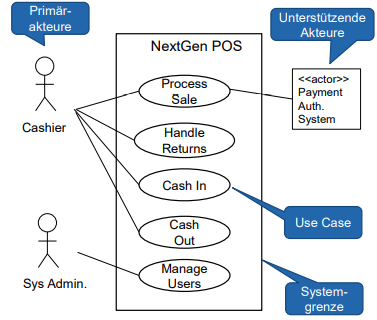
\includegraphics[width=0.3\textwidth] {Resources/Images/UseCaseDiagramm.png}
	\caption{\label{fig:UseCaseDiagramm}UseCaseDiagramm}
	\end{figure}


\title {Zusätzliche Beziehungen im Use Case Diagramm}

\begin{figure}[H]
	\centering
	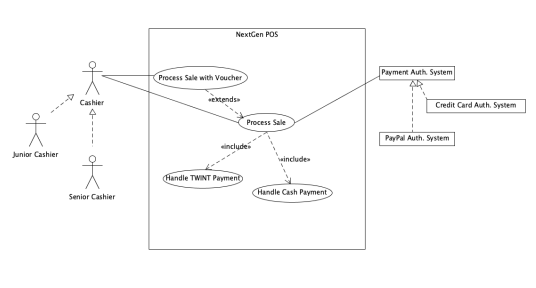
\includegraphics[width=0.3\textwidth] {Resources/Images/UseCaseDiagramm2.png}
	\caption{\label{fig:UseCaseDiagramm2}Zusätzliche Beziehungen UseCaseDiagramm}
	\end{figure}


\subsubsection{UML Sequenzdiagramm (SSD)}


\begin{figure}[H]
	\centering
	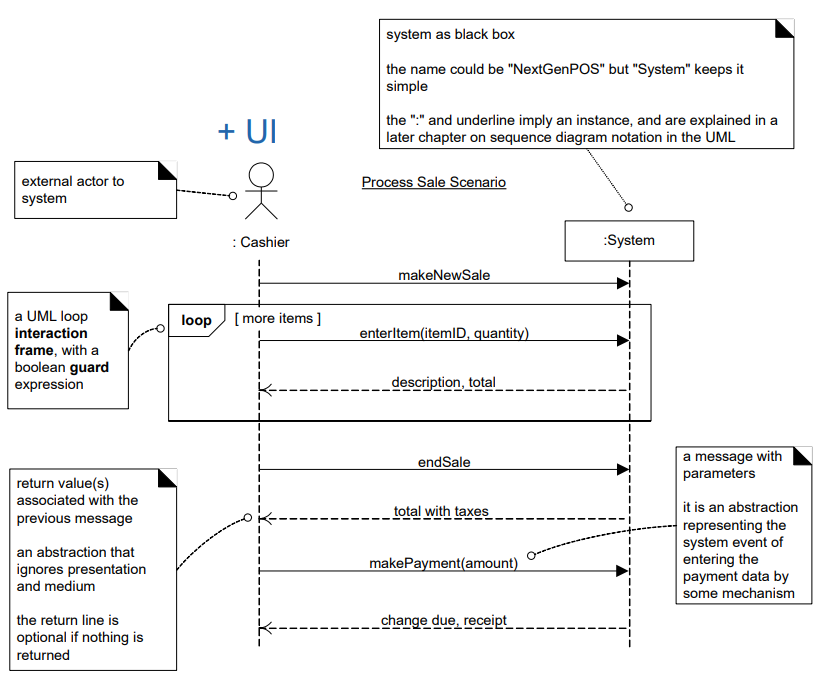
\includegraphics[width=0.3\textwidth] {Resources/Images/Systemsequenzdiagramm.png}
	\caption{\label{fig:Systemsequenzdiagramm}Zusätzliche Beziehungen Systemsequenzdiagramm}
	\end{figure}
	
\title {SSD zwischen zwei Systemen}
\begin{figure}[H]
	\centering
	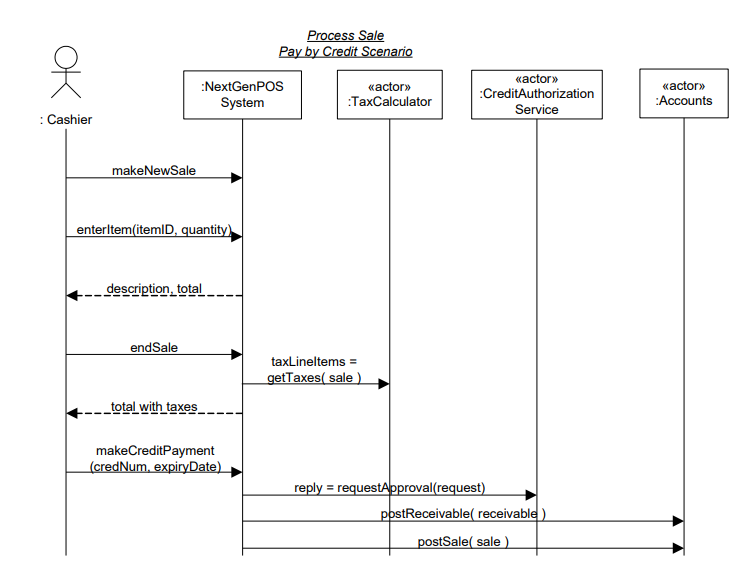
\includegraphics[width=0.3\textwidth] {Resources/Images/SSD2.png}
	\caption{\label{fig:SSD2}Zusätzliche Beziehungen Systemsequenzdiagramm zwischen zwei Systeme}
	\end{figure}

\paragraph{System Operation}
\begin{itemize}
	\item Formal wie ein Methodenaufruf
	\begin{itemize}
		\item Treffender Name
		\item Evt. mit Parametern
		\item Durchzogener Pfeil für Methodenaufruf
		\item Rückgabewert (Kann fehlen falls unwichtig, Gestrichelte Linie weil Update des UI)
		\item Definieren API des Systems
	\end{itemize}

\end{itemize}

\subsubsection{Operation Contract}

\textbf{Definition: } Spezifiziert (System)Operation \\

\begin{itemize}
	\item Name plus Parameterliste
	\item Vorbedingung (Was muss zwingend erfüllt sein damit Systemoperation aufgerufen werden kann)
	\item Nachbedingung
	\begin{itemize}
		\item Was hat sich alles geändert nach Ausführung (Erstellte / gelöschte Instanzen, Assoziationen, geänderte Attribute)
		\item basierend auf Domänenmodell
	\end{itemize}
\end{itemize}

\begin{figure}[H]
	\centering
	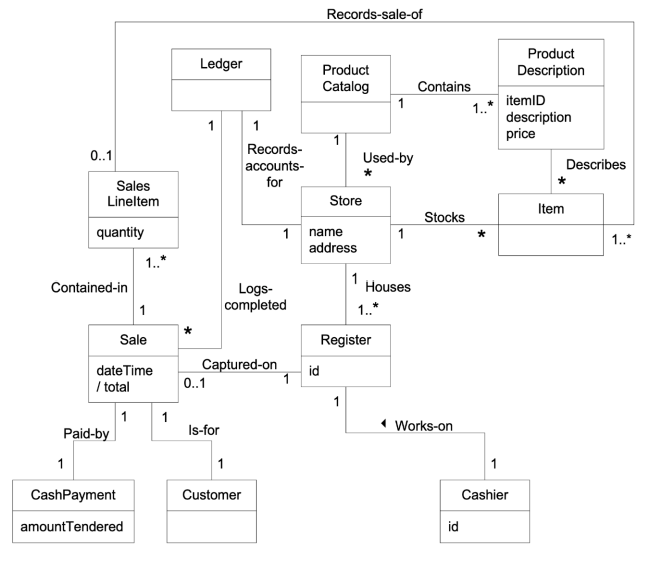
\includegraphics[width=0.3\textwidth] {Resources/Images/OperationContract.png}
	\caption{\label{fig:OperationContract}OperationContract}
	\end{figure}



\subsubsection{Zusätzliche Anforderungen}
\begin{itemize}
	\item Funktionale
	\item Nicht-Funktionale
\end{itemize}


\paragraph{Formulierung}

\begin{itemize}
	\item Anforderungstatements
	\begin{itemize}
		\item Als Anforderung formuliert
		\item messbar/verifizierbar
	\end{itemize}
	\item So wenig wie nötig
	\begin{itemize}
		\item Nur diejenige, die begründet gefordert werden
		\item Keine ersten Lösungsideen als Forderungen
	\end{itemize}
\end{itemize}


\paragraph{Checkliste FURPS+}

\begin{itemize}
	\item \textbf Functionality
	\begin{itemize}
		\item Features, Fähigkeiten, Sicherheit
	\end{itemize}
	\item \textbf Usability
	\begin{itemize}
		\item Usability Anforderungen (Kap.5.3)
		\item Accessibility
	\end{itemize}
	\item \textbf Reliability
	\begin{itemize}
		\item Fehlerrate, Wiederanlauffähigkeit, Vorhersagbarkeit, Datensicherung
	\end{itemize}
	\item \textbf Performance
	\begin{itemize}
		\item Reaktionszeiten, Durchsatz, Genauigkeit, Verfügbarkeit, Ressourceneinsatz
	\end{itemize}
	\item \textbf Supportability
	\begin{itemize}
		\item Anpassungsfähigkeit, Wartbarkeit, Internationalisierung, Konfigurierbarkeit
	\end{itemize}
	\item \textbf {+}
	\begin{itemize}
		\item Implementation (HW,BS,Sprachen, Tests...)
		\item Interface
		\item Operations
		\item Packaging
		\item Legal
	\end{itemize}
\end{itemize}


\paragraph{Glossar}

\begin{itemize}
	\item Einfaches Glossar
	\begin{itemize}
		\item Begriffe im Projekt und SW-Produkt
		\item beliebige Elemente 
	\end{itemize}
	\item Data Dictionary
	\begin{itemize}
		\item Zusätzliche Datenformate, Wertebereiche, Validierungsregeln
	\end{itemize}
\end{itemize}




















































\end{document}